\chapter{绪论}

以下给出一些常用命令。

参考文献引用\cite{abdar_uncertainty_2021, baumgartner_exploration_2018, ackley_learning_1985}

\begin{equation}
    \label{equ:basic_chain_rule}
    \begin{split}
        \frac{\partial L}{\partial \boldsymbol{W_3}} &= \frac{\partial L}{\partial f_3} \cdot \frac{\partial f_3}{\partial \boldsymbol{W_3}} \\
        \frac{\partial L}{\partial \boldsymbol{W_2}} &= \frac{\partial L}{\partial f_3} \cdot \frac{\partial f_3}{\partial f_2} \cdot \frac{\partial f_2}{\partial \boldsymbol{W_2}}  \\
        \frac{\partial L}{\partial \boldsymbol{W_1}} &= \frac{\partial L}{\partial f_3} \cdot \frac{\partial f_3}{\partial f_2} \cdot \frac{\partial f_2}{\partial f_1} \cdot \frac{\partial f_1}{\partial \boldsymbol{W_1}} \\
    \end{split}
\end{equation}

\begin{algorithm}[!ht]
    \caption{反向传播算法}
    \label{alg:basic_back_propagation}

    \KwIn{$l$层神经网络}
    \KwIn{激活函数$f_i \text{, } i\in l$}
    \KwIn{输出数据$\boldsymbol{x}$,真实标签$\boldsymbol{y}$}
    
    计算前向传播:$\boldsymbol{\hat{y}} = f_l \left( \boldsymbol{W_l} \ldots f_2 \left( \boldsymbol{W_2} f_1 \left( \boldsymbol{W_1 x} \right) \right) \right)$
    
    计算输出结果与真实标签之间误差:$L = loss \left( \boldsymbol{\hat{y}}, \boldsymbol{y} \right)$
    
    计算初始梯度:$\delta = \partial L / \partial f_{l}$

    \For{$i$ in $\left[ l, 0, -1 \right]$}
    {
        根据链式法计算损失函数关于第$i$层网络权重$\boldsymbol{W_i}$的偏导:$\partial L / \partial \boldsymbol{W_i} = \delta \cdot \partial f_i / \partial \boldsymbol{W_i}$
        
        使用优化算法对当前层网络权重进行更新,如梯度下降法
        
        将当前梯度反向传播至前一层:$\delta = \delta \cdot \partial f_i / \partial f_{i-1}$
    }
\end{algorithm}

\begin{figure}[!ht]
    \centering
    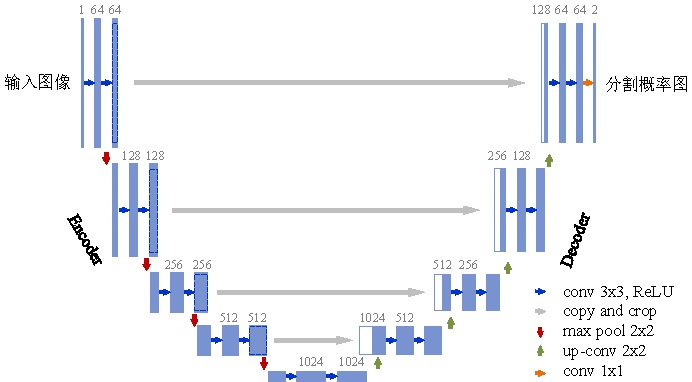
\includegraphics[width=0.9\textwidth]{figure/basic_theory/unet_arch}
    \bicaption{U-Net网络结构}{U-Net architecture}
    \label{fig:basic_unet_arch}
\end{figure}

\begin{figure}
     \centering
     \begin{subfigure}[t]{0.32\textwidth}
         \centering
         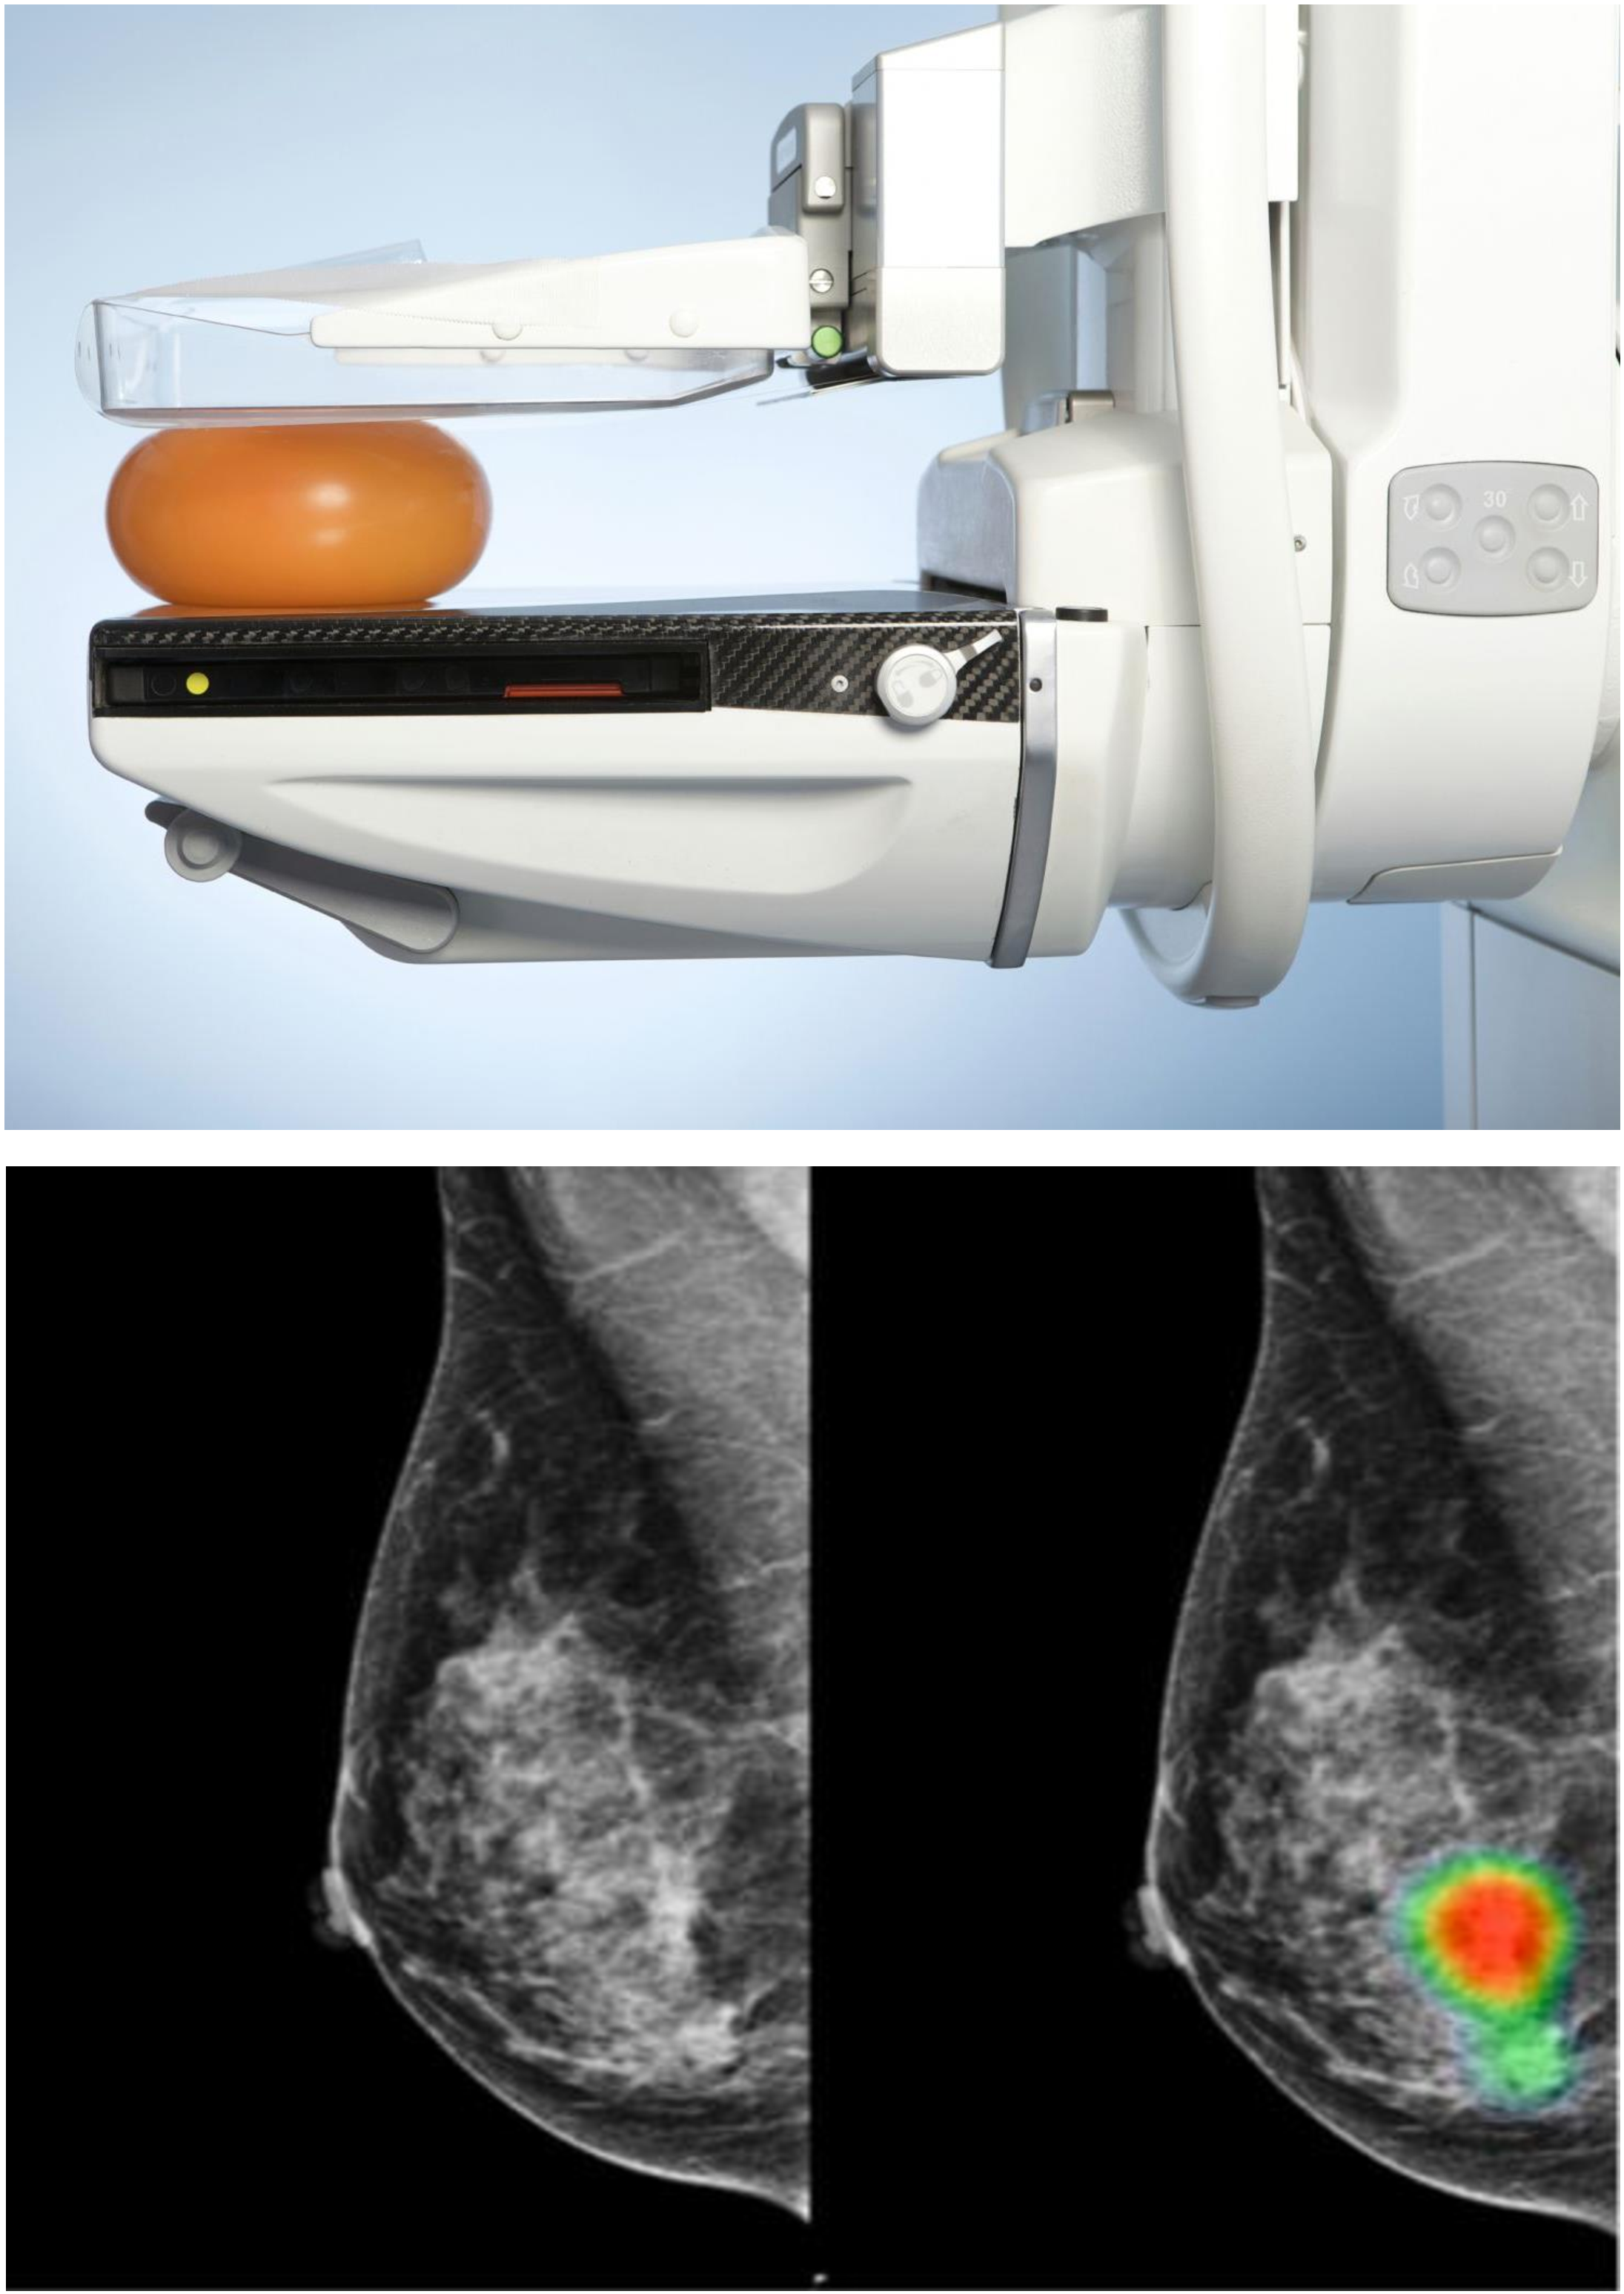
\includegraphics[width=\textwidth]{figure/introdution/mammogram}
         \bicaption{X线钼靶}{Mammography}
         \label{subfig:mammography}
     \end{subfigure}
     \begin{subfigure}[t]{0.32\textwidth}
         \centering
         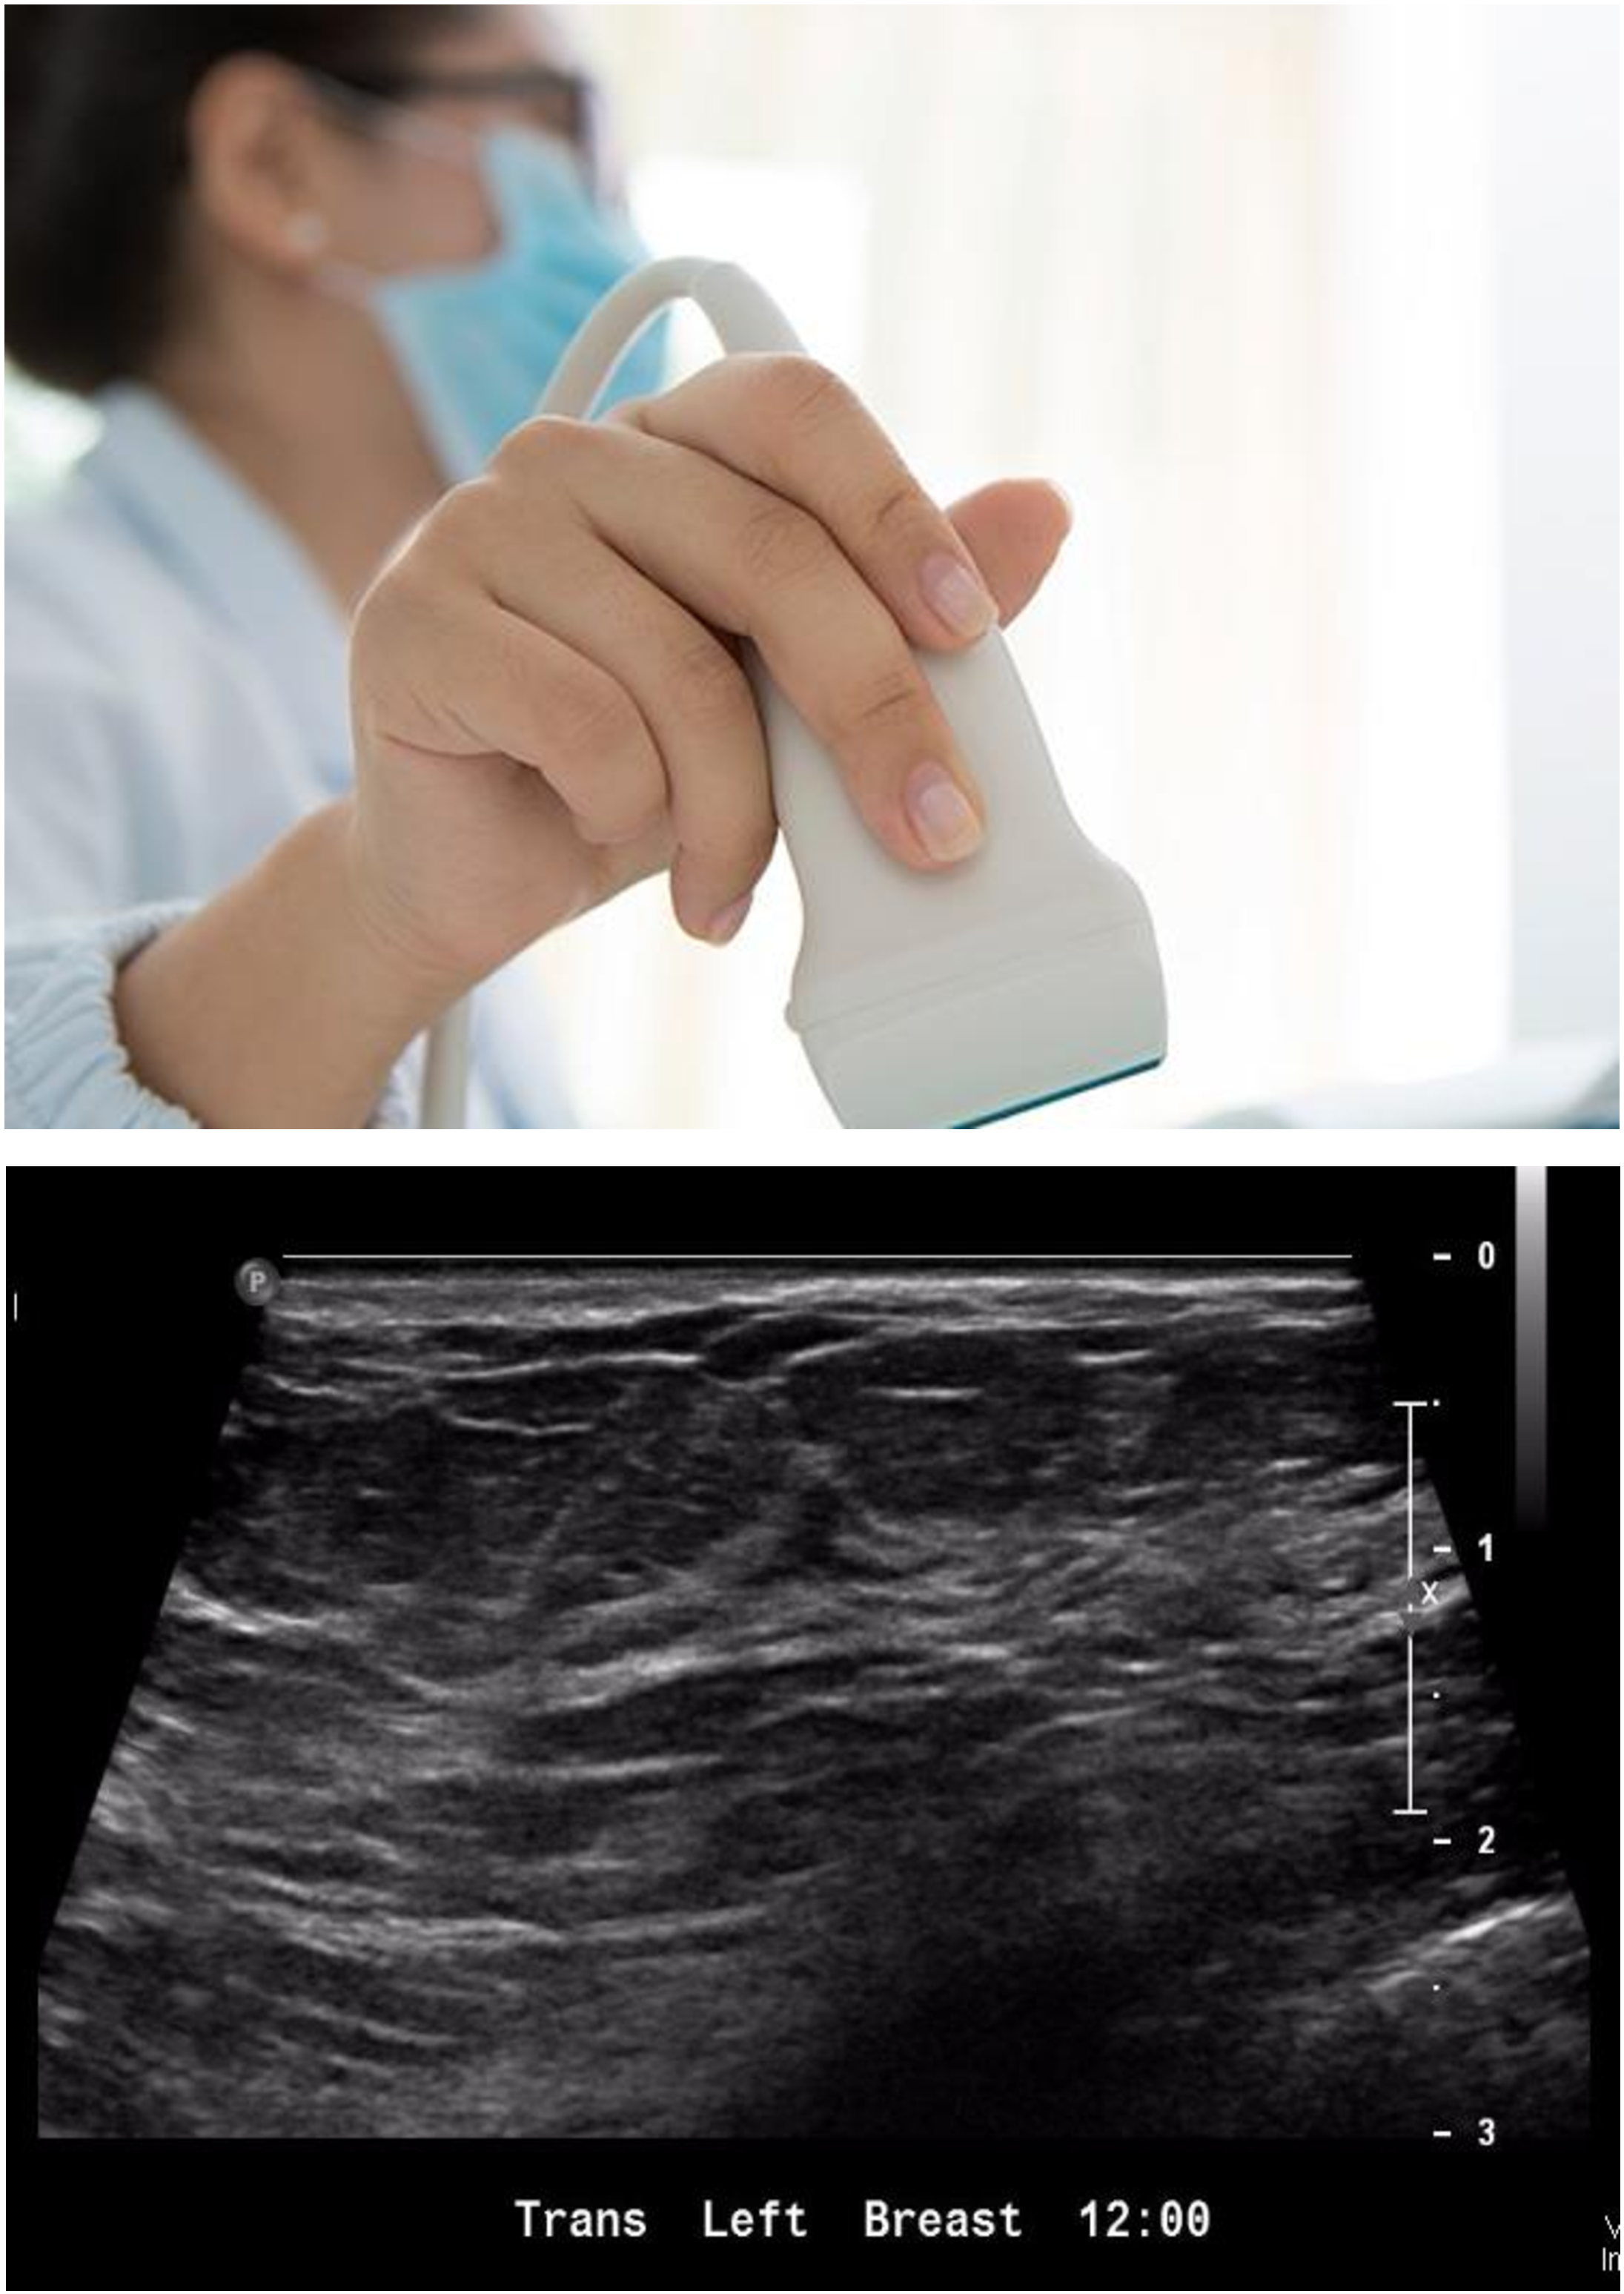
\includegraphics[width=\textwidth]{figure/introdution/bus}
         \bicaption{手动乳腺超声}{Handheld breast ultrasound}
         \label{subfig:bus}
     \end{subfigure}
     \begin{subfigure}[t]{0.32\textwidth}
         \centering
         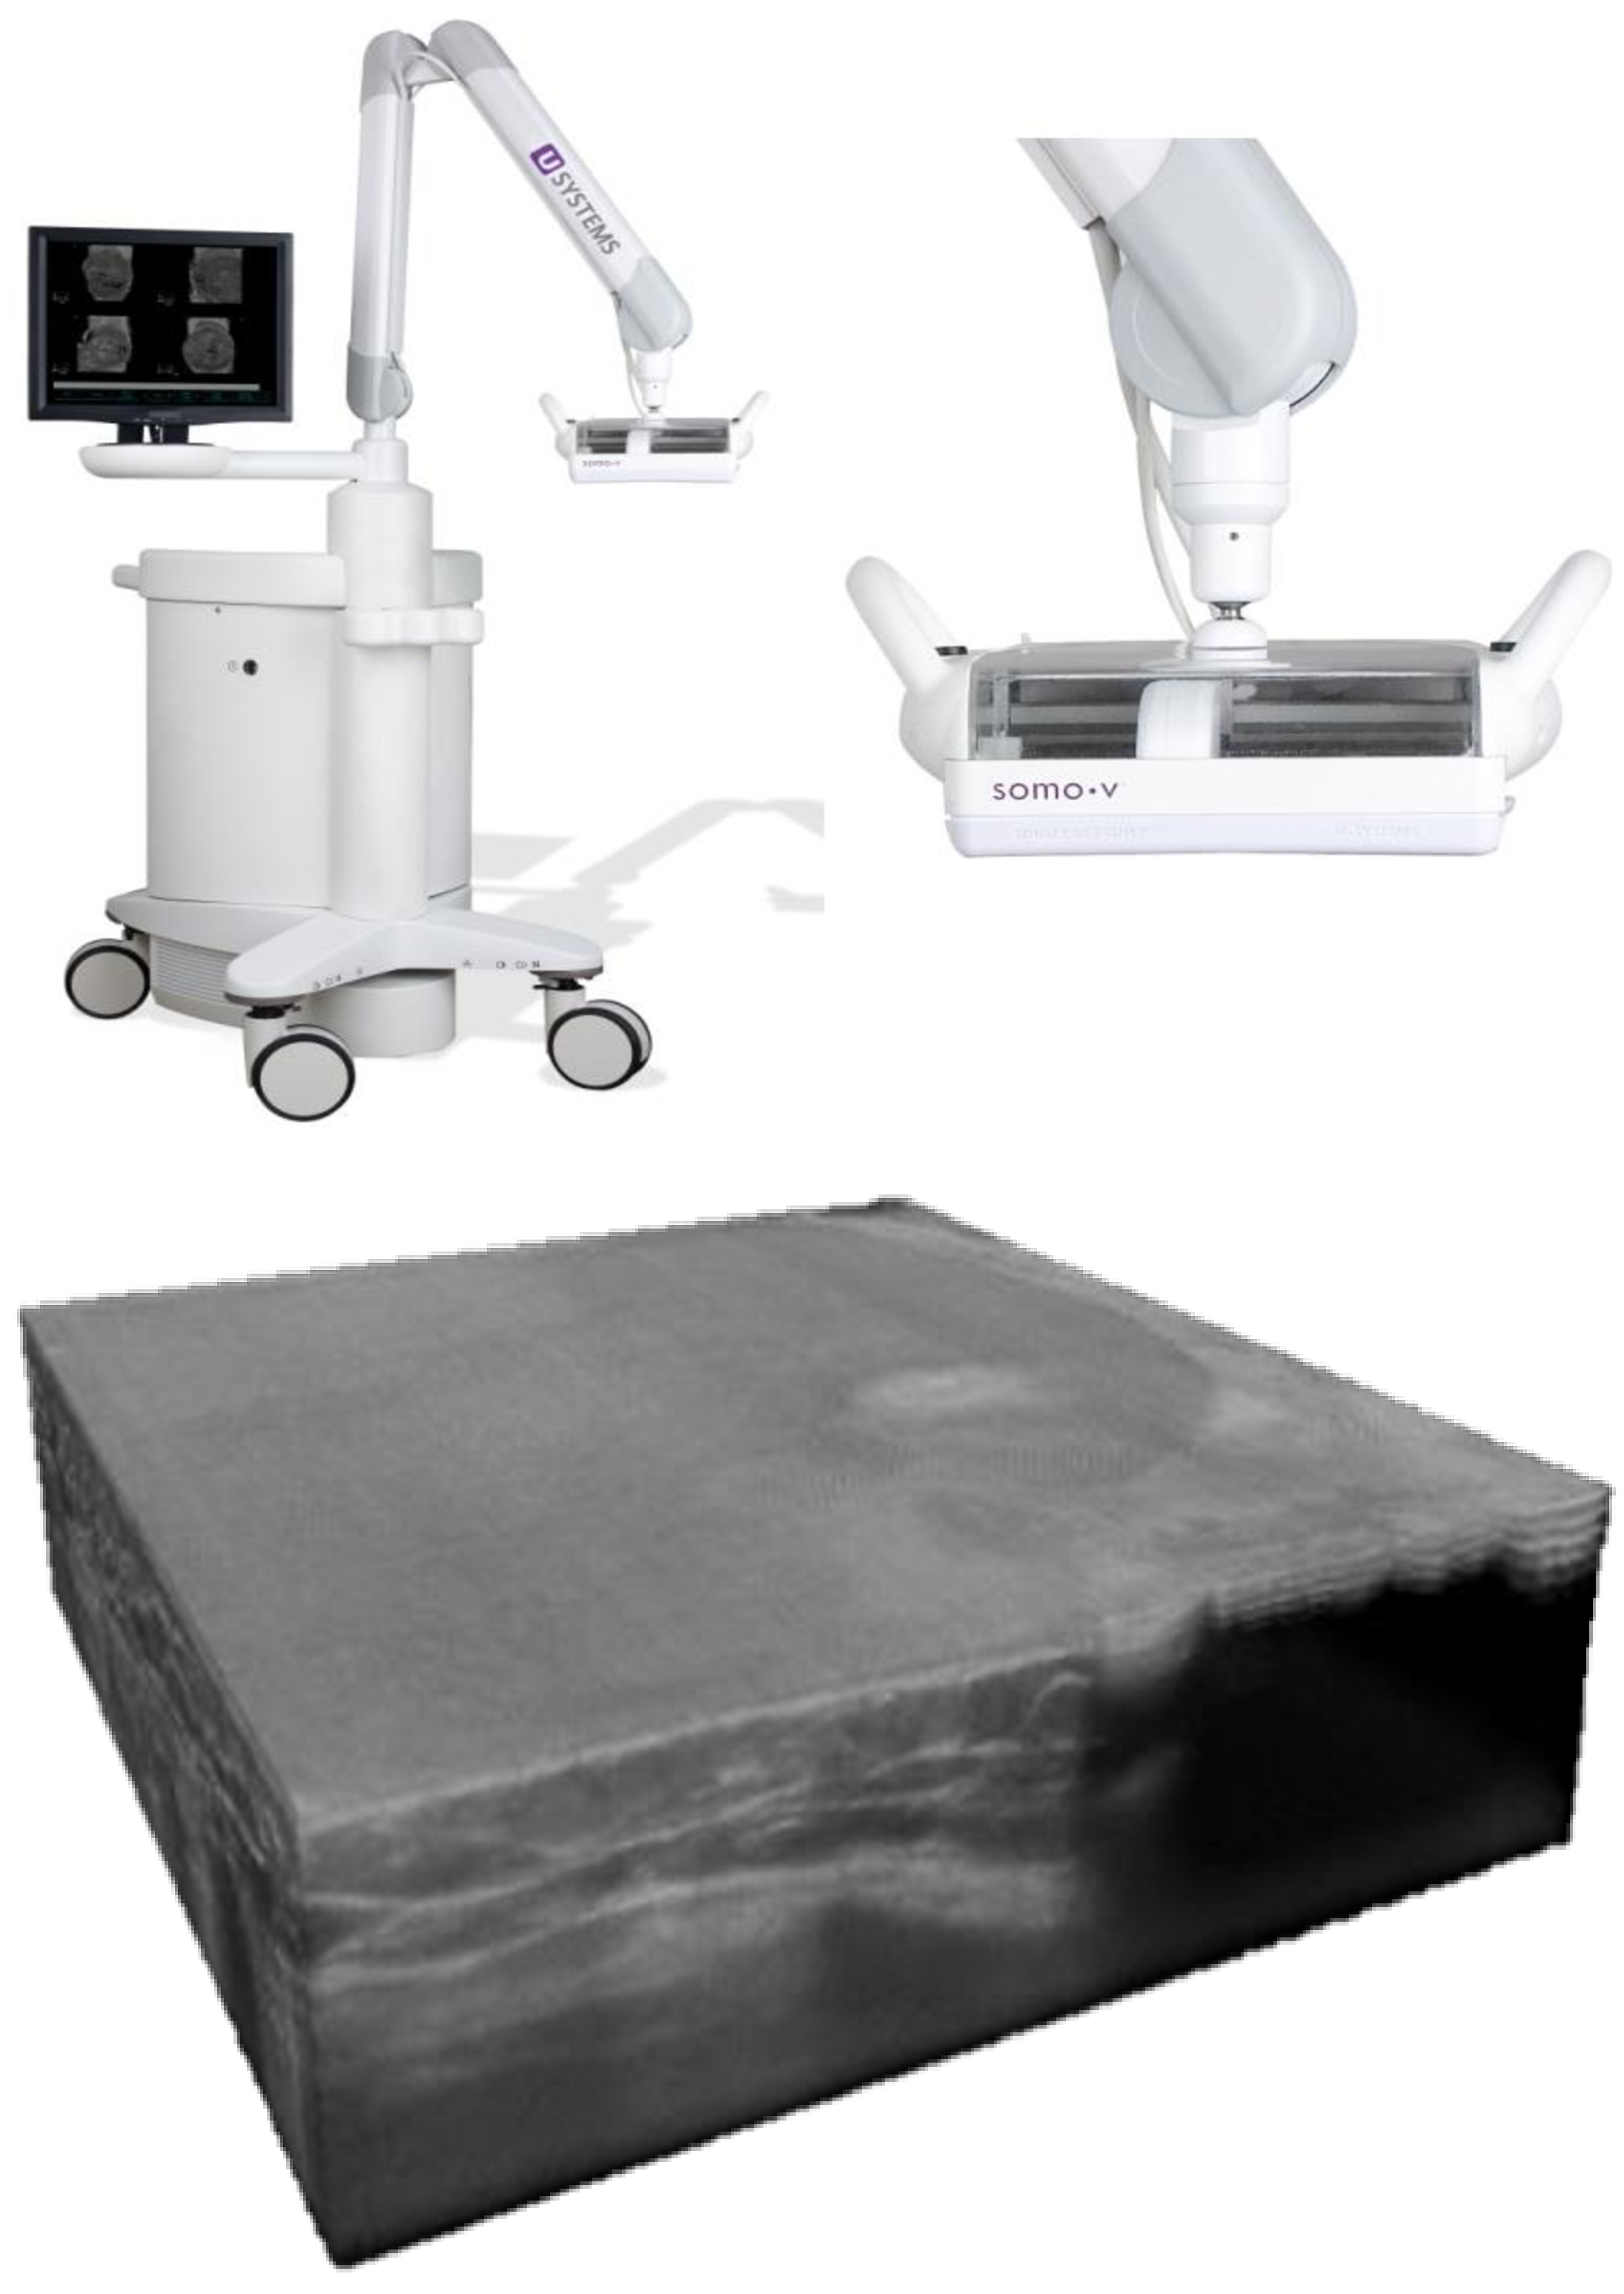
\includegraphics[width=\textwidth]{figure/introdution/abus}
         \bicaption{乳腺自动超声}{Automated breast ultrasound}
         \label{subfig:abus}
     \end{subfigure}
    \bicaption{不同乳腺成像仪器及对应的影像模态}{Different breast imaging scanners and the corresponding imaging modalities}
    \label{fig:intro_diff_imaging_modalities}
\end{figure}

\begin{table}[!ht]
    \bicaption{使用不同数量有标签图像的全监督与半监督分割结果对比}{Quantitative segmentation results of supervised and semi-supervised methods under different numbers of labeled images}
    \centering
    \begin{tabular}{cccccc}
        \toprule
        有标签数量 / 无标签数量 & 方法 & JI &  DSC & Acc & HD \\
        \hline
        100 / 0 & 全监督 & 0.4695 & 0.5871 & 0.9827 & 14.30mm \\
        100 / 8756 & UATE & \textbf{0.5643} & \textbf{0.6727} & \textbf{0.9895} & \textbf{5.95mm}\\
        \hline
        300 / 0 & 全监督 & 0.5407 & 0.6552 & 0.9881 &  9.14mm\\
        300 / 8556 & UATE & \textbf{0.6215} & \textbf{0.7287} & \textbf{0.9910} & \textbf{4.39mm}\\
        \hline
        885 / 0 & 全监督 & 0.5756 & 0.6890 & 0.9897 & 8.06mm\\
        885 / 7971 & UATE & \textbf{0.6270} & \textbf{0.7328} & \textbf{0.9911} & \textbf{4.13mm}\\
        \hline
        1770 / 0 & 全监督 & 0.5933 & 0.7070 & 0.9904 & 7.06mm\\
        1770 / 7086 & UATE & \textbf{0.6316} & \textbf{0.7372} & \textbf{0.9912} & \textbf{3.92mm}\\
        \hline
        4428 / 0 & 全监督 & 0.5961 & 0.7089 & 0.9904 & 8.46mm\\
        4428 / 4428 & UATE & \textbf{0.6365} & \textbf{0.7425} & \textbf{0.9921} & \textbf{3.81mm}\\
        \hline
        8856 / 0 & 全监督 & 0.6078 & 0.7125 & 0.9911 & 5.34mm\\
        \bottomrule
    \end{tabular}
    \label{tab:uate_result_diff_sample_data}
\end{table}

\begin{table}[!ht]
    \centering
    \bicaption{Dense U-Net 网络结构}{Dense U-Net architectures}
    \begin{tiny}
    \begin{tabular}{c|c|c|c|c}
        \toprule
        Layers & Output Size & Dense U-Net 121 & Dense U-Net 161 & Dense U-Net 201 \\
        \hline
        Input Layer & $128\times 512$ & \multicolumn{3}{c}{-}\\
        \hline
        Convolution & $64\times 256$ & \multicolumn{3}{c}{$7\times 7$ conv, stride 2} \\
        \hline
        Pooling & $32 \times 128$ & \multicolumn{3}{c}{$3\times 3$ max pool, stride 2} \\
        \hline
        Dense Block 1 & $32\times 128$ & $\begin{bmatrix}1\times 1 \text{ conv} \\3\times 3 \text{ conv} \end{bmatrix}\times 6$ & $\begin{bmatrix}1\times 1 \text{ conv} \\3\times 3 \text{ conv} \end{bmatrix}\times 6$ & $\begin{bmatrix}1\times 1 \text{ conv} \\3\times 3 \text{ conv} \end{bmatrix}\times 6$\\ 
        \hline
        \multirow{2}{*}{Transition Layer 1} & $32\times 128$ & \multicolumn{3}{c}{$1\times 1$ conv} \\
        \cline{2-5}
         & $16\times 64$ & \multicolumn{3}{c}{$2\times 2$ average pool, stride 2} \\
        \hline
        Dense Block 2 & $16\times 64$ & $\begin{bmatrix}1\times 1 \text{ conv} \\3\times 3 \text{ conv} \end{bmatrix}\times 12$ & $\begin{bmatrix}1\times 1 \text{ conv} \\3\times 3 \text{ conv} \end{bmatrix}\times 12$ & $\begin{bmatrix}1\times 1 \text{ conv} \\3\times 3 \text{ conv} \end{bmatrix}\times 12$ \\
        \hline
        \multirow{2}{*}{Transition Layer 2} & $16\times 64$ & \multicolumn{3}{c}{$1\times 1$ conv} \\
        \cline{2-5}
         & $8\times 32$ & \multicolumn{3}{c}{$2\times 2$ average pool, stride 2} \\
        \hline
        Dense Block 3 & $8\times 32$ & $\begin{bmatrix}1\times 1 \text{ conv} \\3\times 3 \text{ conv} \end{bmatrix}\times 24$ & $\begin{bmatrix}1\times 1 \text{ conv} \\3\times 3 \text{ conv} \end{bmatrix}\times 36$ & $\begin{bmatrix}1\times 1 \text{ conv} \\3\times 3 \text{ conv} \end{bmatrix}\times 48$ \\
        \hline
        \multirow{2}{*}{Transition Layer 3} & $8\times 32$ & \multicolumn{3}{c}{$1\times 1$ conv} \\
        \cline{2-5}
         & $4\times 16$ & \multicolumn{3}{c}{$2\times 2$ average pool, stride 2} \\
        \hline
        Dense Block 4 & $4\times 16$ & $\begin{bmatrix}1\times 1 \text{ conv} \\3\times 3 \text{ conv} \end{bmatrix}\times 16$ & $\begin{bmatrix}1\times 1 \text{ conv} \\3\times 3 \text{ conv} \end{bmatrix}\times 24$ & $\begin{bmatrix}1\times 1 \text{ conv} \\3\times 3 \text{ conv} \end{bmatrix}\times 32$ \\
        \hline
        Up-Sampling Layer 1 & $8\times 32$ & $2\times 2$ upsampling, conv, 512 & $2\times 2$ upsampling, conv, 768 & $2\times 2 $ upsampling, conv, 512 \\
        \hline
        Up-Sampling Layer 2 & $16\times 64$ & $2\times 2$ upsampling, conv, 256 & $2\times 2$ upsampling, conv, 384 & $2\times 2$ upsampling, conv, 256 \\
        \hline
        Up-Sampling Layer 3 & $32\times 128$ & \multicolumn{3}{c}{$2\times 2$ upsampling, conv, 96} \\
        \hline
        Up-Sampling Layer 4 & $64\times 256$ & \multicolumn{3}{c}{$2\times 2$ upsampling, conv, 96} \\
        \hline
        Up-Sampling Layer 5 & $128\times 512$ & \multicolumn{3}{c}{$2\times 2$ upsampling, conv, 64} \\
        \hline
        Output Layer & $128\times 512$ & \multicolumn{3}{c}{$1\times 1$ conv, 2} \\
        \bottomrule
    \end{tabular}
    \end{tiny}
    \label{tab:uate_denseunet_architecture}
\end{table}